\documentclass[a4paper,14pt]{extarticle}

\usepackage[utf8x]{inputenc}
\usepackage[T1,T2A]{fontenc}
\usepackage[russian]{babel}
\usepackage{hyperref}
\usepackage{indentfirst}
\usepackage{here}
\usepackage{array}
\usepackage{graphicx}
\usepackage{caption}
\usepackage{subcaption}
\usepackage{chngcntr}
\usepackage{amsmath}
\usepackage{amssymb}
\usepackage{pgfplots}
\usepackage{pgfplotstable}
\usepackage[left=2cm,right=2cm,top=2cm,bottom=2cm,bindingoffset=0cm]{geometry}
\usepackage{multicol}
\usepackage{askmaps}
\usepackage{titlesec}
\usepackage{listings}
\usepackage{color}
\usepackage{courier}

\definecolor{green}{rgb}{0,0.6,0}
\definecolor{gray}{rgb}{0.5,0.5,0.5}
\definecolor{purple}{rgb}{0.58,0,0.82}

\lstset{
	language=Verilog,
	backgroundcolor=\color{white},   
	basicstyle=\small\ttfamily,
	commentstyle=\color{green},
	keywordstyle=\color{blue},	
	numberstyle=\tiny\color{gray},
	stringstyle=\color{purple},
	breakatwhitespace=false,
	breaklines=true,
	captionpos=b,
	keepspaces=true,
	numbers=left,
	numbersep=5pt,
	showspaces=false,
	showstringspaces=false,
	showtabs=false,
	tabsize=4,
	frame=single,
	inputpath={../quartus/},
	literate={~} {$\sim$}{1}
}

\renewcommand{\le}{\ensuremath{\leqslant}}
\renewcommand{\leq}{\ensuremath{\leqslant}}
\renewcommand{\ge}{\ensuremath{\geqslant}}
\renewcommand{\geq}{\ensuremath{\geqslant}}
\renewcommand{\epsilon}{\ensuremath{\varepsilon}}
\renewcommand{\phi}{\ensuremath{\varphi}}
\renewcommand{\thefigure}{\arabic{figure}} 	
\renewcommand*\not[1]{\overline{#1}}

\titleformat*{\section}{\large\bfseries} 
\titleformat*{\subsection}{\normalsize\bfseries} 
\titleformat*{\subsubsection}{\normalsize\bfseries} 
\titleformat*{\paragraph}{\normalsize\bfseries} 
\titleformat*{\subparagraph}{\normalsize\bfseries} 

\counterwithin{figure}{section}
\counterwithin{equation}{section}
\counterwithin{table}{section}
\newcommand{\sign}[1][5cm]{\makebox[#1]{\hrulefill}}
\graphicspath{{../pics/}}
\captionsetup{justification=centering,margin=1cm}
\def\arraystretch{1.3}
\setlength\parindent{5ex}
\titlelabel{\thetitle.\quad}

\begin{document}

\begin{titlepage}
\begin{center}
	Санкт-Петербургский Политехнический Университет Петра Великого\\[0.3cm]
	Институт компьютерных наук и технологий \\[0.3cm]
	Кафедра компьютерных систем и программных технологий\\[4cm]
	
	\textbf{ОТЧЕТ}\\ 
	\textbf{по лабораторной работе}\\[0.5cm]
	\textbf{SystemVerilog №4}\\[0.1cm]
	Автоматизация проектирования\\ дискретных устройств\\[4.0cm]
\end{center}

\begin{flushright}
	\begin{minipage}{0.45\textwidth}
		\textbf{Работу выполнил студент}\\[3mm]
		группа 33501/4 \hspace*{9mm} Дьячков В.В.\\[5mm]
		\textbf{Преподаватель}\\[5mm]
		\sign[1.5cm] \hspace*{1mm} к.т.н., доц. Филиппов А.С. \\[5mm]
	\end{minipage}
\end{flushright}

\vfill

\begin{center}
	Санкт-Петербург\\
	\the\year
\end{center}
\end{titlepage}

\addtocounter{page}{1}
\counterwithin{lstlisting}{section}

\tableofcontents
\newpage
\listoffigures
\lstlistoflistings
\newpage

\section{lab1\_1}

\subsection{Задание}

На языке Verilog опишите устройство, обеспечивающее:
\begin{itemize}
	\item Управление включением светодиодов \verb|led[7:0]| от соответствующих переключателей (\verb|sw[7:0]|).
	\item При нажатии на кнопку \verb|pba|, сигнал, передаваемый с переключателей к светодиодам, инвертируется.
	\item При нажатии на кнопку \verb|p	bb| все светодиоды должны быть включены (независимо от положения переключателей \verb|sw[7:0]| и кнопки \verb|pba|).
\end{itemize}

В описании можно использовать операторы Bitwise, Logical, Reduction. Тип данных - wire.

\subsection{Код на языке Verilog}

В листинге \ref{code:1} приведен код программы на языке Verilog.

\lstinputlisting[caption=lab1\_1.v, label=code:1]{lab1_1/lab1_1.v}

\newpage

\subsection{Результаты синтеза}

На рис. \ref{fig:lab1_1_rtl} приведено изображение синтезированной схемы в RLT Viewer.

\begin{figure}[H]
\begin{center}
	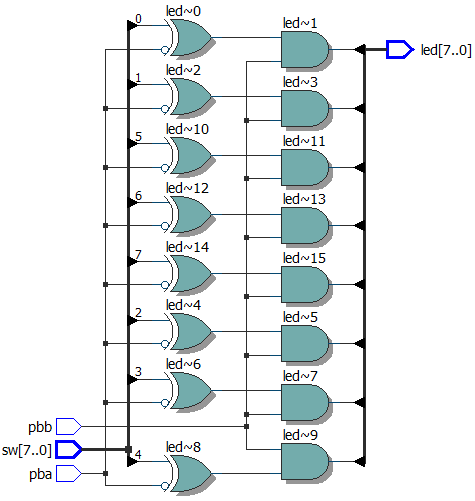
\includegraphics[scale=0.8]{lab1_1_rtl}
	\caption{Результат синтеза в RLT Viewer}
	\label{fig:lab1_1_rtl}
\end{center}
\end{figure}

\subsection{Результаты моделирования}
\label{sec:lab1_1_modeling}

На рис. \ref{fig:lab1_1_modeling} изображена временная диаграмма работы синтезированного устройства. На вход устройству поочередно подаются всевозможные комбинации \code{pba} и \code{pbb}.
\begin{figure}[H]
\begin{center}
	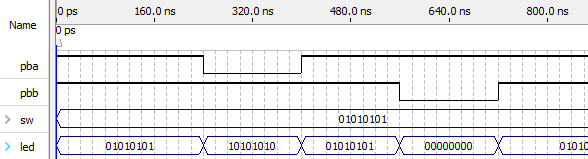
\includegraphics[width=\textwidth]{lab1_1_modeling}
	\caption{Результаты моделирования}
	\label{fig:lab1_1_modeling}
\end{center}
\end{figure}
Из результатов моделирования видно, что при неактивных \code{pba} и \code{pbb} светодиоды \code{led} полностью повторяют значения переключателей \code{sw}; при активном \code{pba} и неактивном \code{pbb} сигнал с переключателей инвертируется; при активном уровне \code{pbb} независимо от значения \code{pba} светодиоды будут включены.

\subsection{Назначение выводов СБИС}

На рис. \ref{fig:lab1_1_pins} приведены назначения выводов СБИС в Pin Planner.

\begin{figure}[H]
\begin{center}
	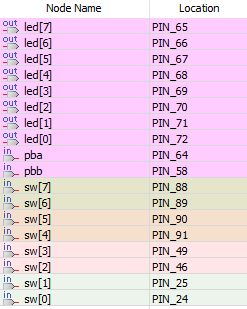
\includegraphics{lab1_1_pins}
	\caption{Таблица назначений в Pin Planer}
	\label{fig:lab1_1_pins}
\end{center}
\end{figure}

\subsection{Результаты проверки на плате}

Для тестирования проекта на плате были использованы тесты, описанные в пункте \ref{sec:lab1_1_modeling}. Результаты тестирования совпадают с ожидаемыми, следовательно, устройство работает верно.

\subsection{Выводы}

Разработано устройство, обеспечивающее управление светодиодами при помощи переключателей. В описании использовались Bitwise операторы. Результаты моделирования и тестирования на плате показали, что разработанное устройство работает верно.

\newpage

\section{lab1\_2}

\subsection{Задание}

На языке Verilog опишите мультиплексор 2 (4 бит) $\rightarrow$ 1 (4 бит):
\begin{itemize}
	\item Входы данных переключатели \code{sw[7:4]} и \code{sw[3:0]} соответственно.
	\item Выходы – светодиоды \code{led[3:0]}
	\item Управление переключением – кнопка \code{pba}:
		\begin{itemize}
			\item \code{pba = 1}: \code{sw[7:4]} $\rightarrow$ \code{led[3:0]}
			\item \code{pba = 0}: \code{sw[3:0]} $\rightarrow$ \code{led[3:0]}
		\end{itemize}
\end{itemize}

В описании можно использовать операторы Bitwise, Logical, Reduction, Replicator, Concatenate.

\subsection{Код на языке Verilog}

В листинге \ref{code:2} приведен код программы на языке Verilog.

\lstinputlisting[caption=lab1\_2.v, label=code:2]{lab1_2/lab1_2.v}

\newpage

\subsection{Результаты синтеза}

На рис. \ref{fig:lab1_2_rtl} приведено изображение синтезированной схемы в RLT Viewer.

\begin{figure}[H]
\begin{center}
	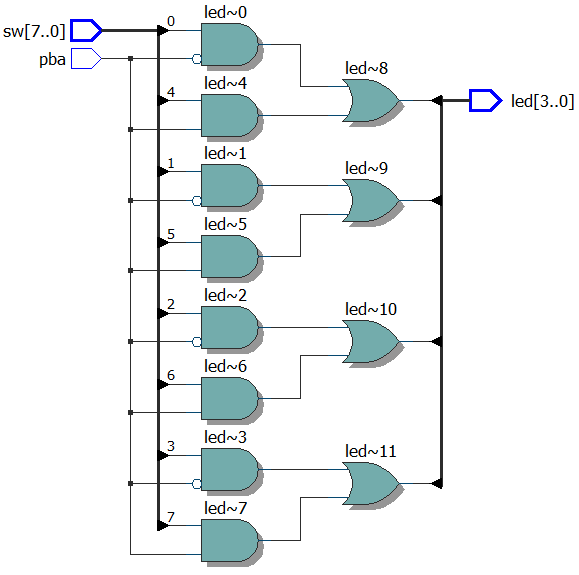
\includegraphics[scale=0.65]{lab1_2_rtl}
	\caption{Результат синтеза в RLT Viewer}
	\label{fig:lab1_2_rtl}
\end{center}
\end{figure}

\subsection{Результаты моделирования}
\label{sec:lab1_2_modeling}

На рис. \ref{fig:lab1_2_modeling} изображена временная диаграмма работы синтезированного устройства. На вход устройству поочередно подаются всевозможные комбинации \code{pba}.
\begin{figure}[H]
\begin{center}
	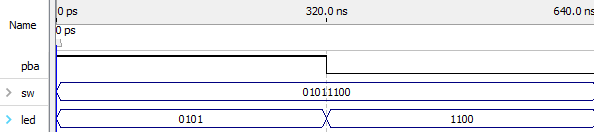
\includegraphics[width=\textwidth]{lab1_2_modeling}
	\caption{Результаты моделирования}
	\label{fig:lab1_2_modeling}
\end{center}
\end{figure}
Из результатов моделирования видно, что при \code{pba=1} значения \code{led=sw[7:4]}, а при \code{pba=0} значения \code{led=sw[3:0]}.

\subsection{Назначение выводов СБИС}

На рис. \ref{fig:lab1_2_pins} приведены назначения выводов СБИС в Pin Planner.

\begin{figure}[H]
\begin{center}
	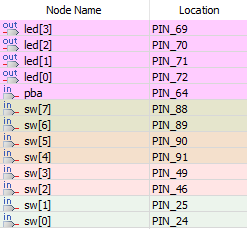
\includegraphics{lab1_2_pins}
	\caption{Таблица назначений в Pin Planer}
	\label{fig:lab1_2_pins}
\end{center}
\end{figure}

\subsection{Результаты проверки на плате}

Для тестирования проекта на плате были использованы тесты, описанные в пункте \ref{sec:lab1_2_modeling}. Результаты тестирования совпадают с ожидаемыми, следовательно, устройство работает верно.

\subsection{Выводы}

Разработан мультиплексор 2 $\rightarrow$ 1. В описании использовались такие операторы, как Bitwise, Replicator. Результаты моделирования и тестирования на плате показали, что разработанное устройство работает верно.

\newpage

\section{lab1\_3}

\subsection{Задание}

На языке Verilog опишите демультиплексор 1 (2 бит) $\rightarrow$ 4 (2 бит):
\begin{itemize}
	\item Входы данных - переключатели \code{sw[1:0]} соответственно.
	\item Выходы – светодиоды \code{led[7:0]}.
	\item Управление демультиплексором – кнопки \code{pba} и \code{pbb}.
\end{itemize}

В описании можно использовать операторы Bitwise, Logical, Reduction, Replicator, Concatenate.

\subsection{Код на языке Verilog}

В листинге \ref{code:3} приведен код программы на языке Verilog.

\lstinputlisting[caption=lab1\_3.v, label=code:3]{lab1_3/lab1_3.v}

\newpage

\subsection{Результаты синтеза}

На рис. \ref{fig:lab1_3_rtl} приведено изображение синтезированной схемы в RLT Viewer.

\begin{figure}[H]
\begin{center}
	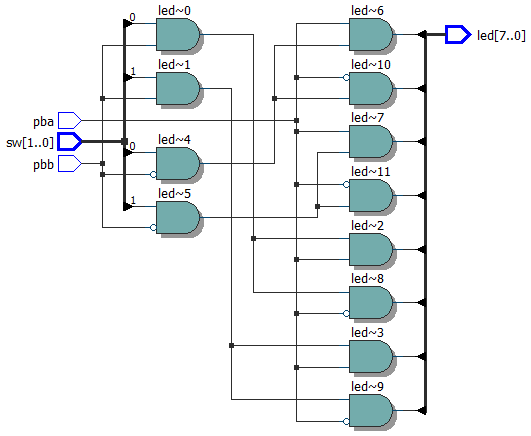
\includegraphics[scale=0.9]{lab1_3_rtl}
	\caption{Результат синтеза в RLT Viewer}
	\label{fig:lab1_3_rtl}
\end{center}
\end{figure}

\subsection{Результаты моделирования}
\label{sec:lab1_3_modeling}

На рис. \ref{fig:lab1_3_modeling} изображена временная диаграмма работы синтезированного устройства. На вход устройству поочередно подаются всевозможные комбинации \code{pba} и \code{pbb}.
\begin{figure}[H]
\begin{center}
	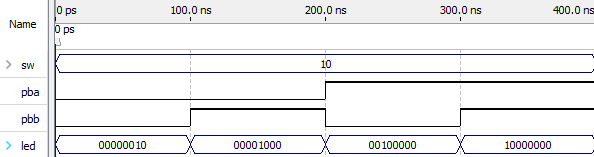
\includegraphics[width=\textwidth]{lab1_3_modeling}
	\caption{Результаты моделирования}
	\label{fig:lab1_3_modeling}
\end{center}
\end{figure}

\subsection{Назначение выводов СБИС}

На рис. \ref{fig:lab1_3_pins} приведены назначения выводов СБИС в Pin Planner.

\begin{figure}[H]
\begin{center}
	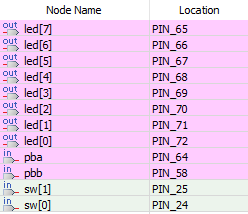
\includegraphics{lab1_3_pins}
	\caption{Таблица назначений в Pin Planer}
	\label{fig:lab1_3_pins}
\end{center}
\end{figure}

\subsection{Результаты проверки на плате}

Для тестирования проекта на плате были использованы тесты, описанные в пункте \ref{sec:lab1_3_modeling}. Результаты тестирования совпадают с ожидаемыми, следовательно, устройство работает верно.

\subsection{Выводы}

Разработан демультиплексор 1 $\rightarrow$ 4. В описании использовались такие операторы, как Bitwise и Replicator. Результаты моделирования и тестирования на плате показали, что разработанное устройство работает верно.

\newpage

\section{lab1\_4}

\subsection{Задание}

На языке Verilog опишите преобразователь позиционного кода (1 из N) в двоичный код:
\begin{itemize}
	\item Входы данных переключатели \code{sw[3:0]} соответственно.
	\item Выходы – светодиоды \code{led[1:0]}.
\end{itemize}
В описании можно использовать операторы Bitwise, Logical, Reduction, Replicator, Concatenate.

\subsection{Код на языке Verilog}

В листинге \ref{code:4} приведен код программы на языке Verilog.

\lstinputlisting[caption=lab1\_4.v, label=code:4]{lab1_4/lab1_4.v}

\subsection{Результаты синтеза}

На рис. \ref{fig:lab1_4_rtl} приведено изображение синтезированной схемы в RLT Viewer.

\begin{figure}[H]
\begin{center}
	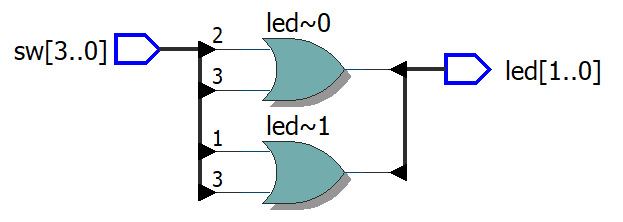
\includegraphics[scale=0.55]{lab1_4_rtl}
	\caption{Результат синтеза в RLT Viewer}
	\label{fig:lab1_4_rtl}
\end{center}
\end{figure}

\subsection{Результаты моделирования}
\label{sec:lab1_4_modeling}

На рис. \ref{fig:lab1_4_modeling} изображена временная диаграмма работы синтезированного устройства. На вход устройству поочередно подаются всевозможные комбинации четырехразрядного позиционного кода \code{sw[3:0]}.
\begin{figure}[H]
\begin{center}
	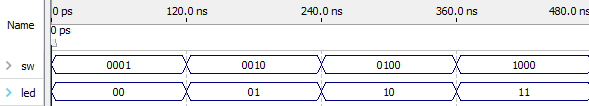
\includegraphics[width=\textwidth]{lab1_4_modeling}
	\caption{Результаты моделирования}
	\label{fig:lab1_4_modeling}
\end{center}
\end{figure}

\subsection{Назначение выводов СБИС}

На рис. \ref{fig:lab1_4_pins} приведены назначения выводов СБИС в Pin Planner.

\begin{figure}[H]
\begin{center}
	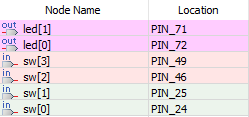
\includegraphics{lab1_4_pins}
	\caption{Таблица назначений в Pin Planer}
	\label{fig:lab1_4_pins}
\end{center}
\end{figure}

\subsection{Результаты проверки на плате}

Для тестирования проекта на плате были использованы тесты, описанные в пункте \ref{sec:lab1_4_modeling}. Результаты тестирования совпадают с ожидаемыми, следовательно, устройство работает верно.

\subsection{Выводы}

Разработан преобразователь позиционного кода в двоичный. В описании использовались такие операторы, как Bitwise и Concatenate. Результаты моделирования и тестирования на плате показали, что разработанное устройство работает верно.

\newpage

\section{lab1\_5}

\subsection{Задание}

На языке Verilog опишите преобразователь двоичного кода в позиционный код (один-из-N):
\begin{itemize}
	\item Входы двоичных данных переключатели \code{sw[1:0]}.
	\item Выходы – светодиоды \code{led[3:0]}.
\end{itemize}
В описании можно использовать операторы Bitwise, Logical, Reduction, Replicator, Concatenate.

\subsection{Код на языке Verilog}

В листинге \ref{code:5} приведен код программы на языке Verilog.

\lstinputlisting[caption=lab1\_5.v, label=code:5]{lab1_5/lab1_5.v}

\subsection{Результаты синтеза}

На рис. \ref{fig:lab1_5_rtl} приведено изображение синтезированной схемы в RLT Viewer.

\begin{figure}[H]
\begin{center}
	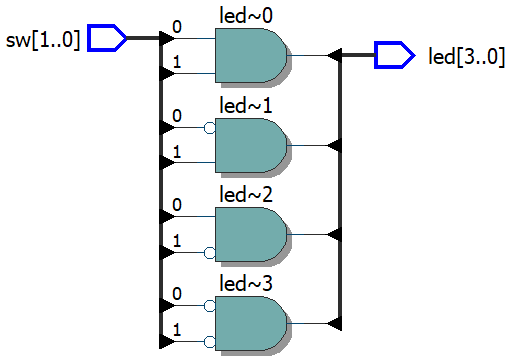
\includegraphics[scale=0.55]{lab1_5_rtl}
	\caption{Результат синтеза в RLT Viewer}
	\label{fig:lab1_5_rtl}
\end{center}
\end{figure}

\subsection{Результаты моделирования}
\label{sec:lab1_5_modeling}

На рис. \ref{fig:lab1_5_modeling} изображена временная диаграмма работы синтезированного устройства. На вход устройству поочередно подаются всевозможные комбинации 2-разрядного двоичного кода \code{sw[1:0]}.
\begin{figure}[H]
\begin{center}
	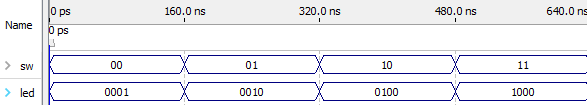
\includegraphics[width=\textwidth]{lab1_5_modeling}
	\caption{Результаты моделирования}
	\label{fig:lab1_5_modeling}
\end{center}
\end{figure}

\subsection{Назначение выводов СБИС}

На рис. \ref{fig:lab1_5_pins} приведены назначения выводов СБИС в Pin Planner.

\begin{figure}[H]
\begin{center}
	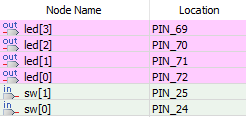
\includegraphics{lab1_5_pins}
	\caption{Таблица назначений в Pin Planer}
	\label{fig:lab1_5_pins}
\end{center}
\end{figure}

\subsection{Результаты проверки на плате}

Для тестирования проекта на плате были использованы тесты, описанные в пункте \ref{sec:lab1_5_modeling}. Результаты тестирования совпадают с ожидаемыми, следовательно, устройство работает верно.

\subsection{Выводы}

Разработан преобразователь двоичного кода в позиционный. В описании использовались такие операторы, как Bitwise, Concatenate. Результаты моделирования и тестирования на плате показали, что разработанное устройство работает верно.

\newpage

\section{elab1\_1}

\subsection{Задание}

На языке Verilog опишите одноразрядный полусумматор:
\begin{itemize}
	\item Входы данных переключатели \code{sw[1:0]}.
	\item Выходы – светодиоды \code{led[1:0]}.
\end{itemize}
В описании можно использовать операторы Bitwise, Logical, Reduction, Replicator, Concatenate.

\subsection{Код на языке Verilog}

В листинге \ref{code:6} приведен код программы на языке Verilog.

\lstinputlisting[caption=elab1\_1.v, label=code:6]{elab1_1/elab1_1.v}

\subsection{Результаты синтеза}

На рис. \ref{fig:elab1_1_rtl} приведено изображение синтезированной схемы в RLT Viewer.

\begin{figure}[H]
\begin{center}
	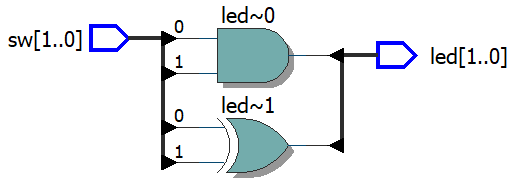
\includegraphics[scale=0.7]{elab1_1_rtl}
	\caption{Результат синтеза в RLT Viewer}
	\label{fig:elab1_1_rtl}
\end{center}
\end{figure}

\subsection{Результаты моделирования}
\label{sec:elab1_1_modeling}

На рис. \ref{fig:elab1_1_modeling} изображена временная диаграмма работы синтезированного устройства. На вход устройству поочередно подаются всевозможные комбинации значений \code{sw}.
\begin{figure}[H]
\begin{center}
	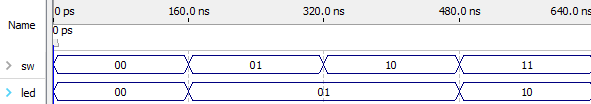
\includegraphics[width=\textwidth]{elab1_1_modeling}
	\caption{Результаты моделирования}
	\label{fig:elab1_1_modeling}
\end{center}
\end{figure}

\subsection{Назначение выводов СБИС}

На рис. \ref{fig:elab1_1_pins} приведены назначения выводов СБИС в Pin Planner.

\begin{figure}[H]
\begin{center}
	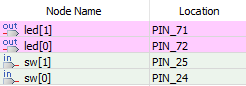
\includegraphics{elab1_1_pins}
	\caption{Таблица назначений в Pin Planer}
	\label{fig:elab1_1_pins}
\end{center}
\end{figure}

\subsection{Результаты проверки на плате}

Для тестирования проекта на плате были использованы тесты, описанные в пункте \ref{sec:elab1_1_modeling}. Результаты тестирования совпадают с ожидаемыми, следовательно, устройство работает верно.

\subsection{Выводы}

Разработан одноразрядный полусумматор. В описании использовались такие операторы, как Bitwise, Concatenate. Результаты моделирования и тестирования на плате показали, что разработанное устройство работает верно.

\newpage

\section{elab1\_2}

\subsection{Задание}

На языке Verilog описать полный одноразрядный сумматор:
\begin{itemize}
	\item Входы:
	\begin{itemize}
		\item Данных - переключатели \code{sw[1:0]}.
		\item Переноса – кнопка \code{pba}.
	\end{itemize}
	\item Выходы – светодиоды \code{led[1:0]}.
\end{itemize}
В описании можно использовать операторы Bitwise, Logical, Reduction, Reduction, Replicator, Concatenate.

\subsection{Код на языке Verilog}

В листинге \ref{code:7} приведен код программы на языке Verilog.

\lstinputlisting[caption=elab1\_2.v, label=code:7]{elab1_2/elab1_2.v}

\subsection{Результаты синтеза}

На рис. \ref{fig:elab1_2_rtl} приведено изображение синтезированной схемы в RLT Viewer.

\begin{figure}[H]
\begin{center}
	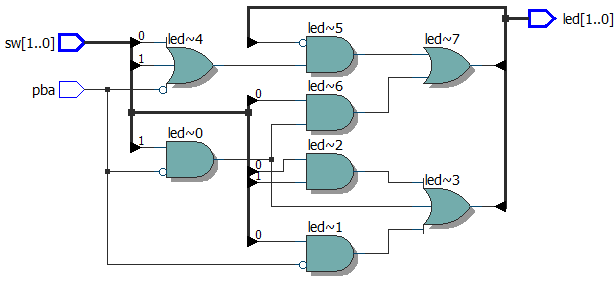
\includegraphics[scale=0.6]{elab1_2_rtl}
	\caption{Результат синтеза в RLT Viewer}
	\label{fig:elab1_2_rtl}
\end{center}
\end{figure}

\subsection{Результаты моделирования}
\label{sec:elab1_2_modeling}

На рис. \ref{fig:elab1_2_modeling} изображена временная диаграмма работы синтезированного устройства. На вход устройству поочередно подаются всевозможные комбинации значений \code{pba} (активный уровень 0) и \code{sw}.
\begin{figure}[H]
\begin{center}
	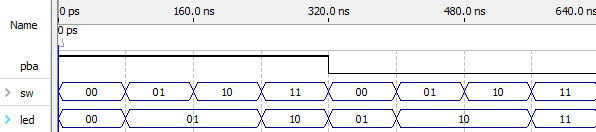
\includegraphics[width=\textwidth]{elab1_2_modeling}
	\caption{Результаты моделирования}
	\label{fig:elab1_2_modeling}
\end{center}
\end{figure}

\subsection{Назначение выводов СБИС}

На рис. \ref{fig:elab1_2_pins} приведены назначения выводов СБИС в Pin Planner.

\begin{figure}[H]
\begin{center}
	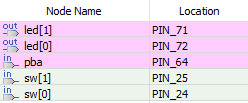
\includegraphics{elab1_2_pins}
	\caption{Таблица назначений в Pin Planer}
	\label{fig:elab1_2_pins}
\end{center}
\end{figure}

\subsection{Результаты проверки на плате}

Для тестирования проекта на плате были использованы тесты, описанные в пункте \ref{sec:elab1_2_modeling}. Результаты тестирования совпадают с ожидаемыми, следовательно, устройство работает верно.

\subsection{Выводы}

Разработан полный одноразрядный сумматор. В описании использовались такие операторы, как Bitwise, Concatenate. Результаты моделирования и тестирования на плате показали, что разработанное устройство работает верно.

\newpage

\section{elab1\_3}

\subsection{Задание}

На языке Verilog опишите полный 2-х разрядный сумматор с последовательным переносом:
\begin{itemize}
	\item Входы:
	\begin{itemize}
		\item Данных - переключатели \code{sw[3:2]} и \code{sw[1:0]} соответственно.
		\item Переноса – кнопка \code{pba}.
	\end{itemize}
	\item Выходы – светодиоды \code{led[2:0]}.
\end{itemize}
В описании можно использовать операторы Bitwise, Logical, Reduction, Reduction, Replicator, Concatenate.

\subsection{Код на языке Verilog}

В листинге \ref{code:8} приведен код программы на языке Verilog.

\lstinputlisting[caption=elab1\_3.v, label=code:8]{elab1_3/elab1_3.v}

\subsection{Результаты синтеза}

На рис. \ref{fig:elab1_3_rtl} приведено изображение синтезированной схемы в RLT Viewer.

\begin{figure}[H]
\begin{center}
	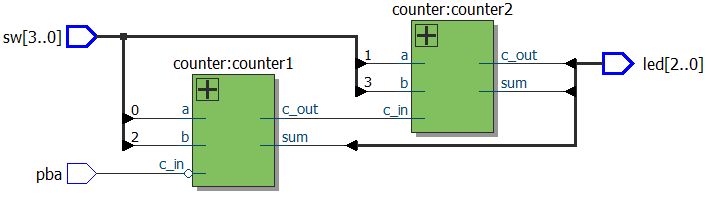
\includegraphics[scale=0.8]{elab1_3_rtl}
	\caption{Результат синтеза в RLT Viewer}
	\label{fig:elab1_3_rtl}
\end{center}
\end{figure}

\subsection{Результаты моделирования}
\label{sec:elab1_3_modeling}

На рис. \ref{fig:elab1_3_modeling} изображены временные диаграммы работы синтезированного устройства. На вход устройству поочередно подаются всевозможные комбинации значений \code{sw} при \code{pba = 1} (неактивный уровень) и при \code{pba = 0} (активный уровень) соответственно.
\begin{figure}[H]
\begin{center}
	\begin{subfigure}[b]{\textwidth}
		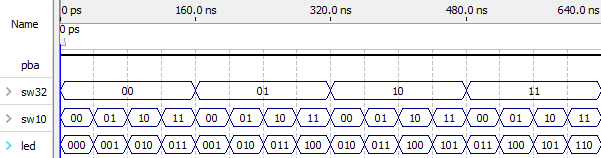
\includegraphics[width=\textwidth]{elab1_3_modeling_1}
	\end{subfigure}
	\begin{subfigure}[b]{\textwidth}
		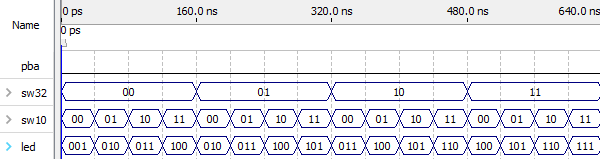
\includegraphics[width=\textwidth]{elab1_3_modeling_2}
	\end{subfigure}
	\caption{Результаты моделирования}
	\label{fig:elab1_3_modeling}
\end{center}
\end{figure}

\subsection{Назначение выводов СБИС}

На рис. \ref{fig:elab1_3_pins} приведены назначения выводов СБИС в Pin Planner.

\begin{figure}[H]
\begin{center}
	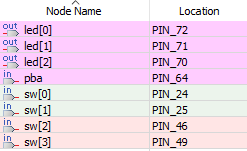
\includegraphics{elab1_3_pins}
	\caption{Таблица назначений в Pin Planer}
	\label{fig:elab1_3_pins}
\end{center}
\end{figure}

\subsection{Результаты проверки на плате}

Для тестирования проекта на плате были использованы тесты, описанные в пункте \ref{sec:elab1_3_modeling}. Результаты тестирования совпадают с ожидаемыми, следовательно, устройство работает верно.

\subsection{Выводы}

Разработан полный 2-х разрядный сумматор с последовательным переносом. В описании использовались такие операторы, как Bitwise, Concatenate. Результаты моделирования и тестирования на плате показали, что разработанное устройство работает верно.

\end{document}